\cleardoublepage

\section{曲线重建}

曲线重建主要分为两个部分,一个是连续化,即将离散的数据连续化;
另一部分是重建,根据连续的数据得到绝对坐标系下的曲线各点坐标。
根据传感器的种类不同,所测得的数据类型不同,这两步工作的执行顺序也可以不同。

如MEMS惯性传感器主要测量加速度数据,并对加速度数据进行二次积分而得到测量点位移,
故可以在计算测量点坐标之后再进行连续化;而像FBG传感器所得到的是测量点的曲率数据,
难以直接计算获得该点坐标,必须先对曲率数据进行连续化,然后再计算得出各点的坐标。

本文主采用更高精度、基于曲率数据的曲线重建方案。故可选用FBG传感器并假定可测得数据为两个正交方向的曲率。

\subsection{连续化}
图形学上常用的连续化算法(曲线)有贝塞尔(Bezier)曲线、B样条曲线、Catmull Rom样条曲线等;
而统计学上常用线性插值、多项式插值等。图形学连续化的常见目的是得到光滑曲线,而统计学则追求最小偏差。
由于“曲率光滑程度对曲线重建结果的影响”尚无理论研究,也超出了本文的研究范围,故本文采用其中最简便的线性插值法。

\subsection{重建}
常用的重建算法有基于Cartesian坐标系的拟合算法和基于Frenet坐标系的拟合算法。
其中Cartesian坐标系下的拟合算法拥有更高精度,而Frenet坐标系下的拟合算法更易于编程计算。
本文提出了一种结合Cartesian坐标系和Frenet标架上两种重建算法的改良算法,
兼具重建精度高和运行速度快的优点,并在附件一中给出了其在Rust编程语言上的实现。

\subsection{重建效果与误差分析}

本结主要内容是重建算法的效果展示与误差分析。
为了方便画图和分析,所用曲线为二维标准余弦曲线。

\subsubsection{结果与误差}

图 ~\ref{fig:cos} 为标准余弦曲线与插值步长为$0.01$时的重建结果对比图。
图 ~\ref{fig:cos-error} 展示了根据横坐标$x$变化的重建误差,误差定义为两曲线$y$轴坐标之差的绝对值。

由图可知标准余弦曲线一个周期内的重建误差都在$0.05$以内。


\begin{figure}[H]
\centering
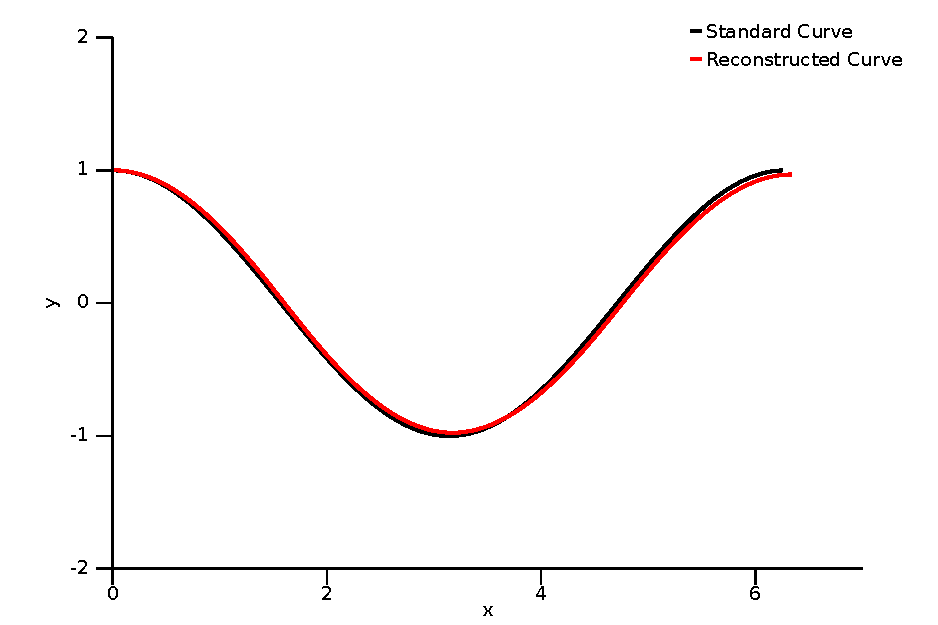
\includegraphics{cos.pdf}
\caption{余弦曲线重建结果}
\label{fig:cos}
\end{figure}

\begin{figure}[H]
\centering
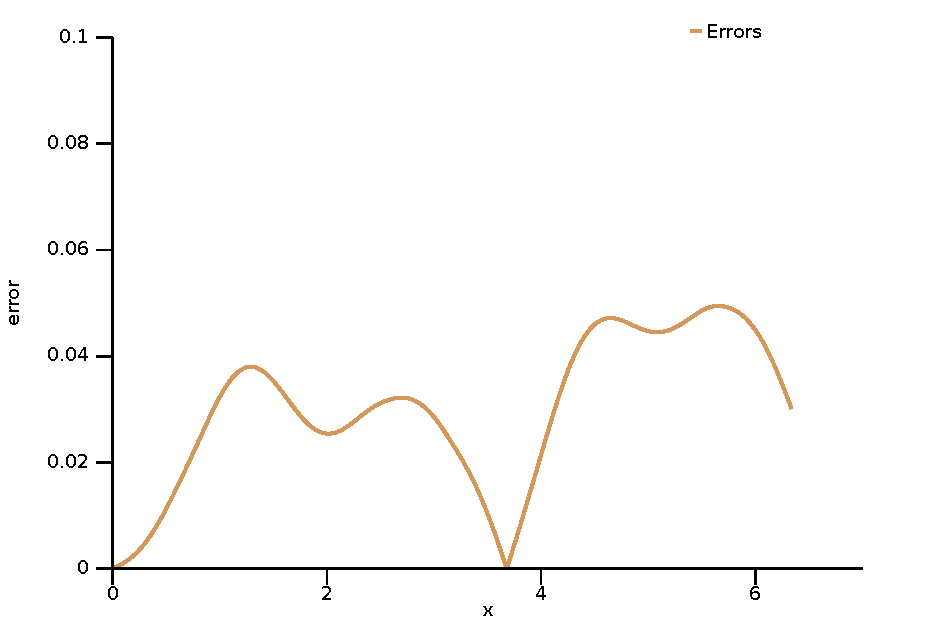
\includegraphics{cos-error.pdf}
\caption{余弦曲线重建误差}
\label{fig:cos-error}
\end{figure}

\subsubsection{不同步长下的误差}

图 ~\ref{fig:cos-diff-step} 为标准余弦曲线与不同插值步长的重建结果对比图。
图 ~\ref{fig:cos-diff-step-error} 展示了横坐标$x$变化下不同插值步长的重建误差。

可知步长越小重建误差越小,但步长从$0.01$减少到$0.001$带来的准确性提升并不是很明显,却增加了十倍的计算负担,
故可认为$0.01$为最适插值步长。

\begin{figure}[H]
\centering
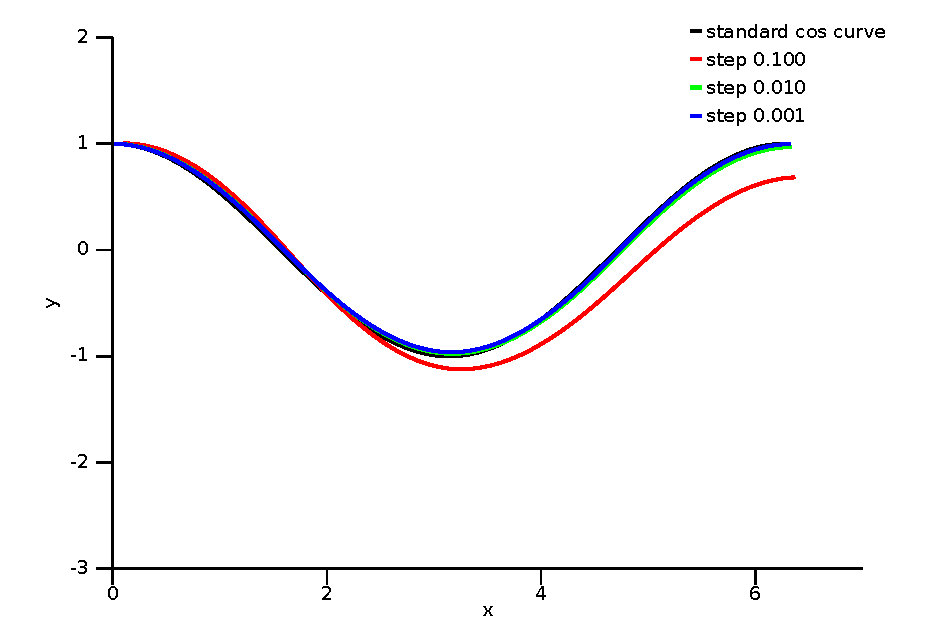
\includegraphics{cos-diff-step.pdf}
\caption{不同步长下的重建结果}
\label{fig:cos-diff-step}
\end{figure}

\begin{figure}[H]
\centering
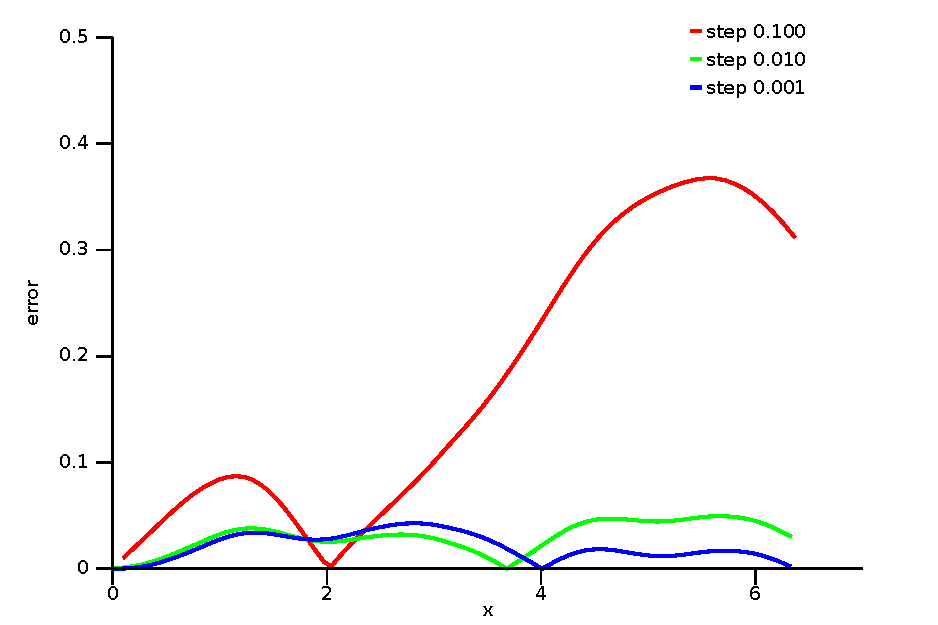
\includegraphics{cos-diff-step-error.pdf}
\caption{不同步长下的重建误差}
\label{fig:cos-diff-step-error}
\end{figure}

\subsubsection{误差传递}

图 ~\ref{fig:cos-single-error-view} 为$x = \frac{\pi}{4}$处加入不同曲率数据误差的重建结果,曲率误差的定义为原始曲率的倍数。
图 ~\ref{fig:cos-single-error} 展示了横坐标$x$变化下加入单点曲率误差的的重建误差传递。

可知单点曲率误差越大重建误差也越大,
且每增加$0.1$倍的曲率误差对重建结果的影响都是巨大的,故原始曲率数据的准确性十分重要。

\begin{figure}[H]
\centering
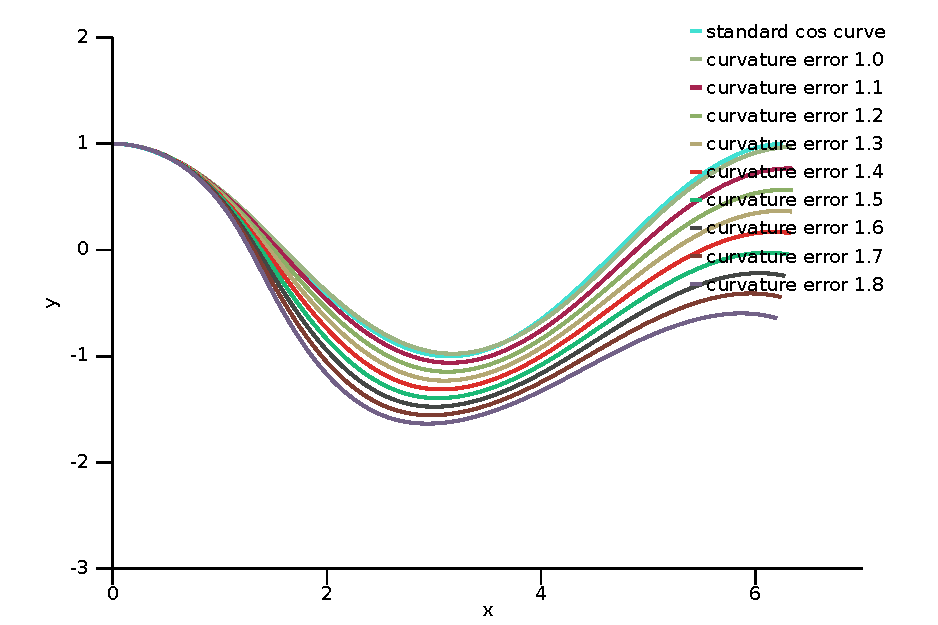
\includegraphics{cos-single-error-view.pdf}
\caption{加入单点误差的重建结果}
\label{fig:cos-single-error-view}
\end{figure}

\begin{figure}[H]
\centering
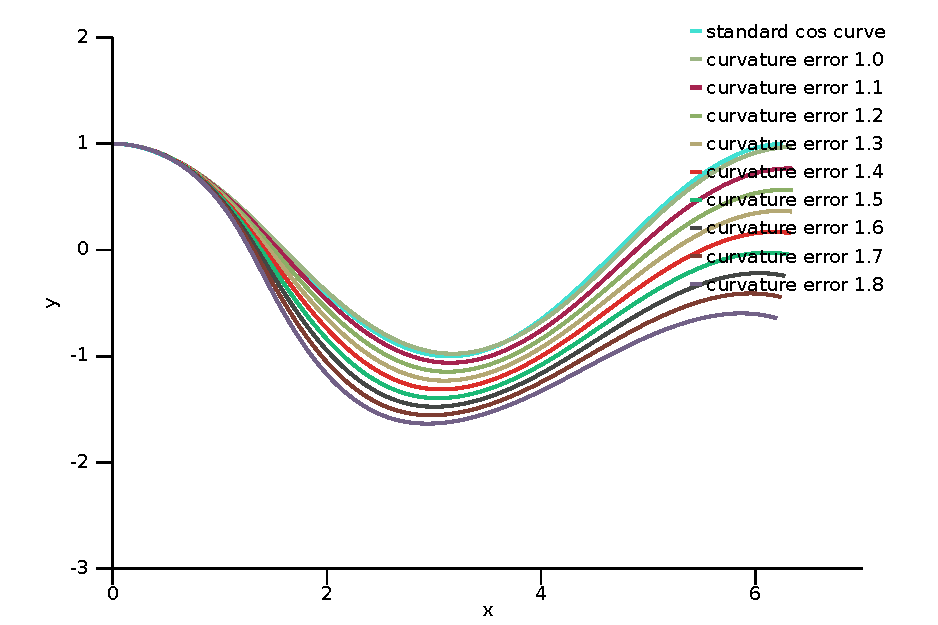
\includegraphics{cos-single-error.pdf}
\caption{单点误差的传递}
\label{fig:cos-single-error}
\end{figure}

图 ~\ref{fig:cos-multiple-error-view} 为曲线上多点分别加入$1.2$曲率数据误差的重建结果。
图 ~\ref{fig:cos-multiple-error} 展示了横坐标$x$变化下分别加入多点曲率误差的的重建误差传递。

可知$s=4.672$处引入曲率误差对重建结果的影响最小,而$s=0.000$处引入对整体曲线影响最大,
但$s=3.820$处引入对后半段曲线的重建结果影响最大,总体来说没什么规律可循。

\begin{figure}[H]
\centering
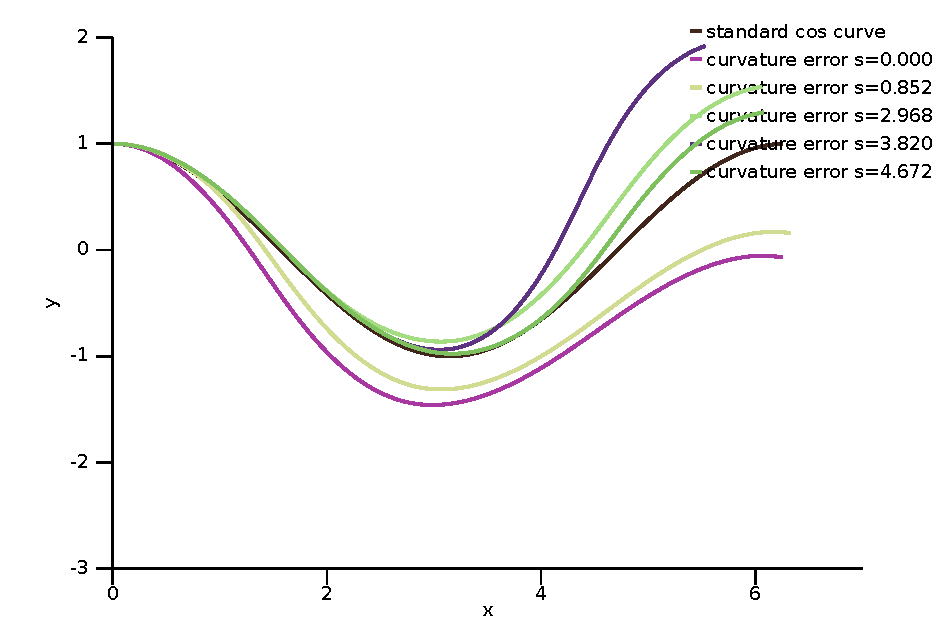
\includegraphics{cos-multiple-error-view.pdf}
\caption{加入多点误差的重建结果}
\label{fig:cos-multiple-error-view}
\end{figure}

\begin{figure}[H]
\centering
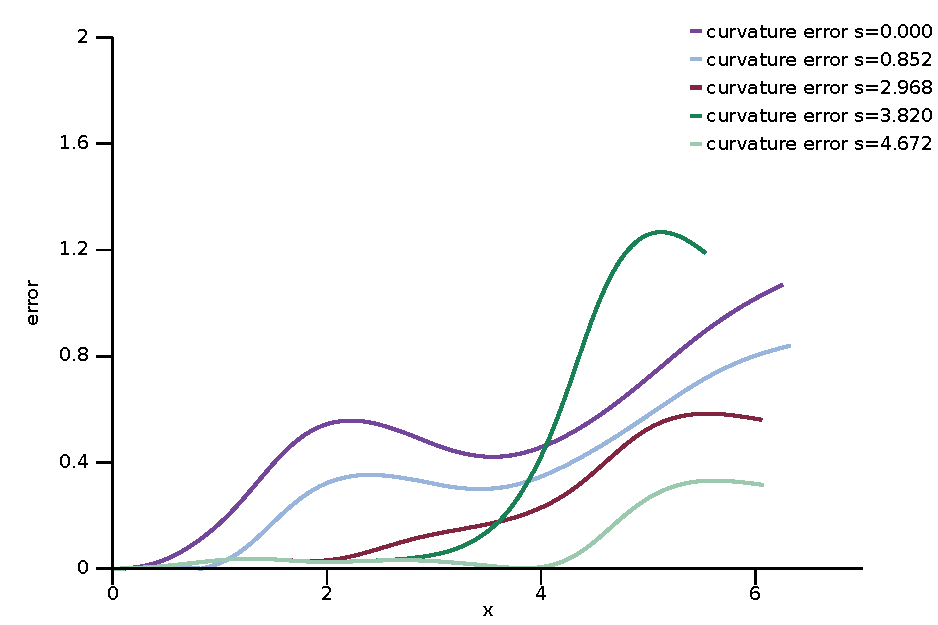
\includegraphics{cos-multiple-error.pdf}
\caption{多点误差的传递}
\label{fig:cos-multiple-error}
\end{figure}

\section{数据传输}

数据传输也主要分为两个部分:一是传感客户端到服务端的原始数据上推流;二是服务器到渲染客户端的重建数据下推流。

所用技术栈有两个选择,一是基于HTTPS的WebSocket,二是基于HTTP2的gRPC。
它们同样是纯流式、高性能且安全。从性能上来说,gRPC略高于WebSocket;
从技术发展上来说,gRPC比WebSocket领先一代。
可惜gRPC-web过于新潮而不被很多后端语言所支持,故本文选择WebSocket on HTTPS。

\subsection{原始数据上推流}

原始数据上推客户端一般运行在一台直接接收传感器数据的机器上,至少需要支持网络栈上的TCP协议。
推荐使用一台运行Linux系统的树莓派。

首先,客户端对服务器端发起一个WebSocket请求:

\begin{lstlisting}
websocket wss://host:port/upstream/
\end{lstlisting}

连接建立之后服务器端给客户端发一个确认包,以告知注册的频道$id$。

\begin{lstlisting}[language=json,firstnumber=1]
{
    "id": 1
}
\end{lstlisting}

我们采用JSON作为主要的数据传输序列化格式,这段数据告诉客户端注册频道$id$为$1$,数据上推准备已完成。

原始数据上推流中的一份数据样例如下:

\begin{lstlisting}[language=json,firstnumber=1]
{
    "ds": 0.01,
    "samples": [
        [0, 0, 0],
        [4.66, 0.21, 0],
        [9.36, 0.27, 0],
        [14.82, 0.086, 0],
        [19.72, -0.0093, 0],
        [24.74, -0.091, 0],
        [29.95, -0.079, 0]
    ]
}
\end{lstlisting}

其中 $d_s$ 为客户端建议的插值步长,
$samples$ 数组内的每个元素都是一个三元组,其中三个数据分别代表与原点的距离$s$、$a$方向的曲率$k_a$和$b$方向的曲率$k_b$。

\subsection{重建数据下推流}

重建数据下推客户端一般是PC上的浏览器,采用频道订阅模式。

下推客户端同样需要先发起一个WebSocket请求:

\begin{lstlisting}
websocket wss://host:port/downstream/:id
\end{lstlisting}

URI中的$:id$为频道$id$,在上推客户端注册时获得。

重建数据下推流中的一份数据样例如下:

\begin{lstlisting}[language=json,firstnumber=1]
{
    "timestamp": 1595915002,
    "points": [
        [0.009999833069741726,1.0000499486923218,0],
        [0.019999666139483452,0.9999996423721313,0],
        [0.029998499900102615,0.9998496174812317,0],
        [0.03999536111950874,0.9996007680892944,0],
        [0.04998929798603058,0.9992536902427673,0],
        [0.059979379177093506,0.998809278011322,0],
        [0.0699646919965744,0.998268187046051,0],
        [0.07994434982538223,0.9976312518119812,0],
        [0.08991748839616776,0.9968992471694946,0],
        [0.09988325089216232,0.9960729479789734,0],
        [0.10984081774950027,0.9951531291007996,0],
        [0.11978939175605774,0.994140625,0],
        [0.009999833069741726,1.0000499486923218,0],
        ...
    ]
}
\end{lstlisting}

其中$timestamp$是数据产生时的时间戳,$points$数组内的每个元素都是一个三元组,
三个数分别是$x$轴、$y$轴和$z$轴的坐标。

\section{三维渲染}

三维渲染采用WebGL渲染引擎和Threejs库,主要功能是根据服务器下推的点列实时渲染管壁或轴线。

WebGL是浏览器上的OpenGL实现,用于在任何兼容的Web浏览器中呈现交互式3D和2D图形\cite{webgl}。
WebGL通过引入一个与OpenGL ES 2.0紧密相符合的API,可以在HTML5 <canvas>元素中使用。

目前支持WebGL的浏览器有:Firefox 4+、Google Chrome 9+、Opera 12+、Safari 5.1+和Internet Explorer 11+;
但是WebGL一些特性也需要用户的硬件设备支持。

WebGL几乎是完全地“跨平台”,使用任何支持WebGL的浏览器打开网页即可完成客户端渲染,而无需下载另外的软件或浏览器插件。

Three.js是一个基于WebGL的3D图形库\cite{threejs},它封装了很多实用的图形组件。

\subsection{轴线渲染}

首先根据下推的点列拟合一条Catmull Rom曲线:

\begin{lstlisting}[language=JavaScript,
   backgroundcolor=\color{lightgray},
   extendedchars=true,
   basicstyle=\footnotesize\ttfamily,
   showstringspaces=false,
   showspaces=false,
   numbers=left,
   numberstyle=\footnotesize,
   numbersep=9pt,
   tabsize=2,
   breaklines=true,
   showtabs=false,
   captionpos=b]

socket.addEventListener('message', event => {
    if (event.data instanceof Blob) {
        event.data.arrayBuffer().then(buffer => {
            let json = inflateRaw(new Uint8Array(buffer), { to: 'string' })
            let data = JSON.parse(json) as Curve
            curve = new THREE.CatmullRomCurve3(data.points.map(
                ({ x, y, z }) => (new Vector3(x, y, z)),
            ))
        }).catch(err => {
            console.log(err)
        })
    }
})
\end{lstlisting}

再定义基础线材质,根据曲线和材质渲染形状并填入缓冲形状:

\begin{lstlisting}[language=JavaScript,
   backgroundcolor=\color{lightgray},
   extendedchars=true,
   basicstyle=\footnotesize\ttfamily,
   showstringspaces=false,
   showspaces=false,
   numbers=left,
   numberstyle=\footnotesize,
   numbersep=9pt,
   tabsize=2,
   breaklines=true,
   showtabs=false,
   captionpos=b]
const material = new THREE.LineBasicMaterial()
const bufGeometry = new THREE.BufferGeometry()
export const object = new THREE.Line(bufGeometry, material)
export const update = () => {
    material.setValues({color: config.color})
    if (curve !== null) {
        bufGeometry.setFromPoints(curve.getPoints(100))
    }
}
\end{lstlisting}

\subsection{管壁渲染}

管壁渲染基于同样的Catmull Rom曲线,但使用网格材质,双边渲染,反光度$100$:

\begin{lstlisting}[language=JavaScript,
   backgroundcolor=\color{lightgray},
   extendedchars=true,
   basicstyle=\footnotesize\ttfamily,
   showstringspaces=false,
   showspaces=false,
   numbers=left,
   numberstyle=\footnotesize,
   numbersep=9pt,
   tabsize=2,
   breaklines=true,
   showtabs=false,
   captionpos=b]
const material = new THREE.MeshPhongMaterial({
    shininess: 100,
    side: THREE.DoubleSide,
})
const bufGeometry = new THREE.BufferGeometry()
export const object = new THREE.Mesh(bufGeometry, material)
export const update = () => {
    material.setValues({color: config.color})
    if (curve !== null) {
        let geometry = new THREE.TubeGeometry(
            curve,
            64,
            0.1,
        )
        bufGeometry.fromGeometry(geometry)
        geometry.dispose()
    }
}
\end{lstlisting}

\subsection{控制器}

主要使用的控制器为轨道控制器,绕原点旋转,启用阻尼:

\begin{lstlisting}[language=JavaScript,
   backgroundcolor=\color{lightgray},
   extendedchars=true,
   basicstyle=\footnotesize\ttfamily,
   showstringspaces=false,
   showspaces=false,
   numbers=left,
   numberstyle=\footnotesize,
   numbersep=9pt,
   tabsize=2,
   breaklines=true,
   showtabs=false,
   captionpos=b]
const orbitControls = new OrbitControls(camera, renderer.domElement)
orbitControls.target = new THREE.Vector3(0, 0, 0)
orbitControls.autoRotate = false
orbitControls.enableDamping = true
orbitControls.dampingFactor = 0.05
\end{lstlisting}

\subsection{环境光}

环境光使用了一个颜色为$\#111111$的全局光和一个颜色为$\#505050$的点光源。

\begin{lstlisting}[language=JavaScript,
   backgroundcolor=\color{lightgray},
   extendedchars=true,
   basicstyle=\footnotesize\ttfamily,
   showstringspaces=false,
   showspaces=false,
   numbers=left,
   numberstyle=\footnotesize,
   numbersep=9pt,
   tabsize=2,
   breaklines=true,
   showtabs=false,
   captionpos=b]
scene.add(new THREE.AmbientLight(0x111111))
let spotLight = new THREE.DirectionalLight(0x505050, 1.5)
spotLight.position.set(0, 1000, 0)
spotLight.castShadow = true
spotLight.shadow.camera.near = 3
spotLight.shadow.camera.far = 10
spotLight.shadow.mapSize.width = 1024
spotLight.shadow.mapSize.height = 1024
scene.add(spotLight)
\end{lstlisting}

\section{软件运行效果}
最终的软件运行效果总体来说很令人满意:运行速度快,稳定60帧渲染;全程TLS加密,安全有保障;
可运行中动态上推、渲染、订阅新的数据源,使用体验极佳。

具体展示见附件二。

\section{总结与展望}
本文总体来说达到了预期目标,使用的也全是当代最先进的技术。
其中WebSocket正支持着成千上万的应用;
TLS保障着整个互联网的安全;
Rust正在为Firefox添砖加瓦;
WebGL定义了下一代的三维渲染程序;
TypeScript是JavaScript社区最受欢迎的转译语言。

从架构方面来说,
渲染任务分离。服务器负责重建,所有的客户端 (浏览器)共享同一份重建数据并渲染。它
大大减少了重建算法的计算压力,仅需一个强有力的服务器完成一次重建,所有的客户端都可以共享重建结果。 
同时,它大大提升了用户的使用体验。在这种架构下,传感器、服务器和客户端即使放置在地球上有互联网覆盖的任意三点,
服务也不会中断。并且终端用户也无需从特定的机器或软件访问服务,而只需要打开任何支持WebGL和TLS
技术的浏览器,即可安全快捷地获得服务。

当然从完成度上来说,这份软件只达到了最小可用的要求,它还需要根据实际需求添加更多的功能以及对现有功能进行调整。
比如添加用户认证系统或者在渲染中更高级的动态分析。

要想构建一个成熟通用的实时三维可视化软件,还有很长的路要走,很多问题有待解决。
